\chapter{Implementation}
\label{chapter:Implementation}

This chapter describes the main modules written by Python and Julia.
The structure of each neural network is also described.


\section{Summary of external modules for this experiments}

\subsection{AutomotiveDrivingModels.jl}

A Julia package containing tools for automotive simulations in 2D.

\subsection{NGSIM.jl}

A Julia package for working with the Next Generation Simulation dataset ({\tt NGSIM}). Was tested on the Highway 101 and I-80 datasets.

This package is fully compatible with {\tt AutomotiveDrivingModels.jl}, providing the {\it Roadway} and {\it Trajdata} types from the {\tt NGSIM} data. Roadway geometry was extracted from the {\tt NGSIM} CAD files. The vehicle trajectories were filtered to provide better global positions and orientation.

The {\tt NGSIM} trajectory data is available in our first release, with instructions here.

\subsection{AutoViz.jl}

A package for rendering simple scenes primarily consisting of cars on roadways using Cairo.

AutoViz is undergoing significant changes.

\begin{figure}[H]
\begin{center}
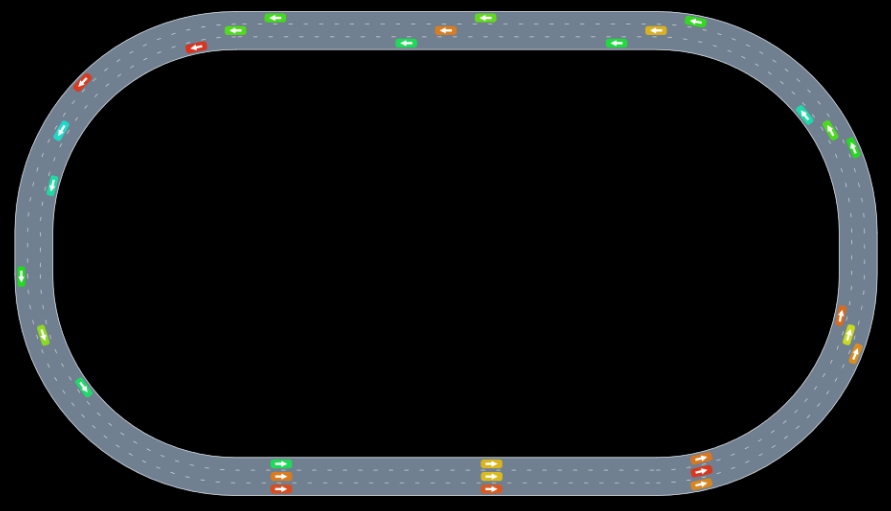
\includegraphics[width=10cm]{./figures/readmeimage.png}
\caption{AutoViz demo.}
\label{fig:example_gridworld}
\end{center}
\end{figure}


\subsection{ForwardNets.jl}

A simple Julia package for neural networks.

\subsection{AutoDrivers.jl}

Advanced human driving models for {\tt AutomotiveDrivingModels.jl}.

\subsection{gail-driver}

Utilities and scripts used to perform experiments described in "Imitating Driver Behavior with Generative Adversarial Networks". Built on rllab and source code for generative adversarial imitation learning.


\subsection{rllab}

{\tt rllab} is a framework for developing and evaluating reinforcement learning algorithms. It includes a wide range of continuous control tasks plus implementations of the following algorithms:

\begin{itemize}
\item    REINFORCE
\item    Truncated Natural Policy Gradient
\item    Reward-Weighted Regression
\item    Relative Entropy Policy Search
\item    Trust Region Policy Optimization
\item    Cross Entropy Method
\item    Covariance Matrix Adaption Evolution Strategy
\item    Deep Deterministic Policy Gradient
\end{itemize}

{\tt rllab} is fully compatible with {\tt OpenAI Gym}. See here for instructions and examples.

{\tt rllab} comes with support for running reinforcement learning experiments on an EC2 cluster, and tools for visualizing the results. See the documentation for details.

The main modules use {\tt Theano} as the underlying framework, and we have support for {\tt TensorFlow} under {\tt sandbox/rocky/tf}.


\section{Software structure summary}

The program is roughly divided into a training program consisting of Python and Julia and a validation program consisting only of Julia.

The following diagrams will be inserted.
\begin{itemize}
\item class diagrams of important classes.
\item relation of data and modules
\end{itemize}




Now writing...


\subsection{Training program summary}

All vehicle behavior is described by the Julia program. The discriminator network is implemented in python's tensorflow.
policy network is a ForwardNets module by Julia, but uses python's tensorflow to configure the network.



\subsection{Validation program summary}

All vehicle behavior is described by the Julia program. 
Policy is also written in Julia.
The validation program does not update Policy. It also doesn't use the discriminator, so it doesn't use Python code.

Now writing...


\section{Features for policy network}


This section details the 51-element input vector used by Policy.

Now writing...

\section{Input for discriminator}


This section details input of discriminator.

Now writing...

\section{Metrics}


This section details the metrics for vehicle behavior that are evaluated by the validation program.

Now writing...

\begin{itemize}
\item Root Weighted Square Error.
\begin{itemize}
\item Position
\item Lane Offset
\item Speed
\end{itemize}
\item Kullback-Leobler Divergence.
\begin{itemize}
\item iTTC
\item Speed
\item Acceleration
\item Turn-Rate
\item Jerk
\end{itemize}
\item Emergent Value.
\begin{itemize}
\item Lane Change Rate
\item Offroad Duration
\item Collision Rate
\item Hard Break Rate
\end{itemize}
\end{itemize}

\section{Summary of environment}

Now writeng...

\begin{itemize}
\item Interstate rode 101 and 80.
\item Data sampling frequency, sampling times.
\end{itemize}


\section{Reward network summary}

Reward network is a discriminator and is realized by tensorflow. The surrogate reward is calculated based on the discrimination result by this network.

\begin{table}[H]
\centering
\begin{tabular}{|c|r|r|}
\hline 
layer  & weight   & bias \\ \hline \hline
input  & 53 x 256 & 256  \\
hidden & 256 x 128 & 128 \\ 
hidden & 128 x 64 & 64 \\ 
hidden & 64 x 64 & 64 \\ 
hidden & 64 x 32 & 32 \\ 
output & 32 x 1 & 1 \\ 
\hline
\end{tabular} 
\caption{}
\label{tab:reward_network}
\end{table}


\begin{itemize}
\item location in sourcecode.
\item specification
\end{itemize}


\section{Policy network summary}


\subsection{GRU structure}


\begin{table}[H]
\centering
\begin{tabular}{|c|r|}
\hline 
layer  & weight    \\ \hline \hline
w\_hc  & 32 x 32   \\
w\_hr  & 32 x 32   \\
w\_hu  & 32 x 32   \\
w\_xc  & 32 x 32   \\
w\_xr  & 32 x 32   \\
w\_xu  & 32 x 32   \\
b\_c  & 32   \\
b\_r  & 32   \\
b\_u  & 32   \\
output & 32 x 2   \\
output bias & 2   \\
\hline
\end{tabular} 
\caption{GRU network gru layer}
\label{tab:reward_gru_gru_network}
\end{table}

\begin{table}[H]
\centering
\begin{tabular}{|c|r|r|}
\hline 
layer  & weight   & bias \\ \hline \hline
input  & 51 x 256 & 256  \\
hidden & 256 x 128 & 128 \\
hidden & 128 x 64  & 64  \\
hidden & 64 x 64   & 64  \\
hidden & 64 x 32   & 32  \\
hidden & 32 x 32   & 32  \\
output & 32 x 2    & 2  \\
\hline
\end{tabular} 
\caption{GRU network mlp layer}
\label{tab:reward_gru_mlp_network}
\end{table}


\begin{itemize}
\item location in sourcecode.
\item specification
\end{itemize}

\subsection{MLP structure}



\begin{table}[H]
\centering
\begin{tabular}{|c|r|r|}
\hline 
layer  & weight   & bias \\ \hline \hline
input  & 51 x 256 & 256  \\
hidden & 256 x 128 & 128 \\
hidden & 128 x 64  & 64  \\
hidden & 64 x 64   & 64  \\
output & 64 x 32   & 32  \\
\hline
\end{tabular} 
\caption{MLP network layer}
\label{tab:reward_mlp_network}
\end{table}



\begin{itemize}
\item location in sourcecode.
\item specification
\end{itemize}

\pagebreak
\section{Summary of environment}

Dataset for this experiment is as follows.

\subsection{Interstate 80 Freeway Dataset(Publication Number: FHWA-HRT-06-137)}


To support the development of microscopic driver behavior algorithms, the Next Generation SIMulation (NGSIM) program is collecting detailed, high-quality traffic datasets. NGSIM stakeholder groups identified the collection of real-world vehicle trajectory data as important to understanding and researching microscopic driver behavior. The NGSIM datasets represent the most detailed and accurate field data collected to date for traffic microsimulation research and development. The Interstate 80 (I-80) freeway dataset was the first of several datasets collected under the NGSIM program.

Researchers for the NGSIM program collected detailed vehicle trajectory data on eastbound I-80 in the San Francisco Bay area in Emeryville, CA, on April 13, 2005. The study area was approximately 500 meters (1,640 feet) in length and consisted of six freeway lanes, including a high-occupancy vehicle (HOV) lane. An onramp also was located within the study area. Seven synchronized digital video cameras, mounted from the top of a 30-story building adjacent to the freeway, recorded vehicles passing through the study area. NG-VIDEO, a customized software application developed for the NGSIM program, transcribed the vehicle trajectory data from the video. This vehicle trajectory data provided the precise location of each vehicle within the study area every one-tenth of a second, resulting in detailed lane positions and locations relative to other vehicles. 

A total of 45 minutes of data are available in the full dataset, segmented into three 15-minute periods: 4:00 p.m. to 4:15 p.m.; 5:00 p.m. to 5:15 p.m.; and 5:15 p.m. to 5:30 p.m. These periods represent the buildup of congestion, or the transition between uncongested and congested conditions, and full congestion during the peak period. In addition to the vehicle trajectory data, the I-80 dataset also contains computer-aided design and geographic information system files, aerial orthorectified photos, freeway loop detector data within and surrounding the study area, raw and processed video, signal timing settings on adjacent arterial roads, traffic sign information and locations, weather data, and aggregate data analysis reports.

The full I-80 dataset is freely available at the NGSIM Web site at \url{http://ops.fhwa.dot.gov/trafficanalysistools/ngsim.htm}.

\begin{figure}[H]
\begin{center}
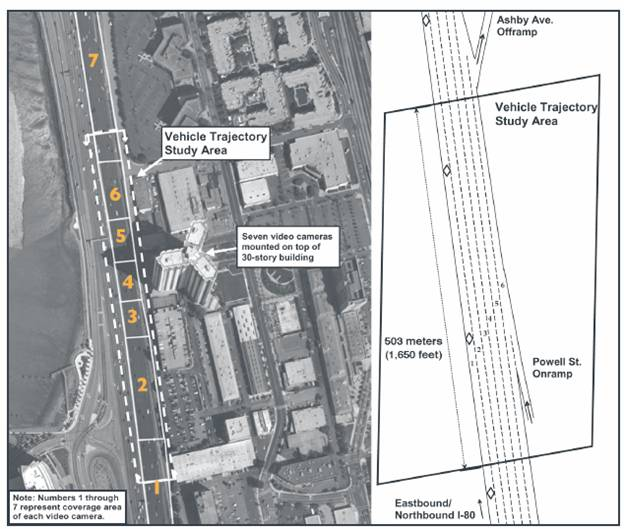
\includegraphics[width=7cm]{./figures/image137b.jpg}
\caption{Interstate 80 Freeway}
\label{fig:pict_us80}
\end{center}
\end{figure}


\subsection{US Highway 101 Dataset(Publication Number: FHWA-HRT-07-030)}

To support the development of algorithms for driver behavior at microscopic levels, the Next Generation SIMulation (NGSIM) computer program is collecting detailed, high-quality traffic datasets. NGSIM stakeholder groups identified the collection of real-world vehicle trajectory data as important to understanding and researching driver behavior at microscopic levels. The NGSIM datasets represent the most detailed and accurate field data collected to date for traffic microsimulation research and development. The US Highway 101 (US 101) dataset was one of several datasets collected under the NGSIM program.
Description

Researchers for the NGSIM program collected detailed vehicle trajectory data on southbound US 101, also known as the Hollywood Freeway, in Los Angeles, CA, on June 15th, 2005. The study area was approximately 640 meters (2,100 feet) in length and consisted of five mainline lanes throughout the section. An auxiliary lane is present through a portion of the corridor between the on-ramp at Ventura Boulevard and the off-ramp at Cahuenga Boulevard. Eight synchronized digital video cameras, mounted from the top of a 36-story building adjacent to the freeway, recorded vehicles passing through the study area. NG-VIDEO, a customized software application developed for the NGSIM program, transcribed the vehicle trajectory data from the video. This vehicle trajectory data provided the precise location of each vehicle within the study area every one-tenth of a second, resulting in detailed lane positions and locations relative to other vehicles.

A total of 45 minutes of data are available in the full dataset, segmented into three 15 minute periods: 7:50 a.m. to 8:05 a.m.; 8:05 a.m. to 8:20 a.m.; and 8:20 a.m. to 8:35 a.m.

These periods represent the buildup of congestion, or the transition between uncongested and congested conditions, and full congestion during the peak period. In addition to the vehicle trajectory data, the US 101 dataset also contains computer-aided design and geographic information system files, aerial ortho-rectified photos, loop detector data, raw and processed video, weather data, and aggregate data analysis reports.

The full US 101 dataset is freely available at the NGSIM Web site at \url{http://ops.fhwa.dot.gov/trafficanalysistools/ngsim.htm}.

Travelers in freeway merge areas face complex tasks in executing their short term trip plans. They must accelerate to the predominant through speeds, check for acceptable gaps, and position themselves for their next maneuvers. During medium and heavy congestion, these tasks are complicated by the volume of other travelers competing for space on crowded freeways.

In reality, travelers often overcome some of this complexity by cooperating with other drivers. Existing microsimulation models generally use basic or modified versions of lane changing models to model freeway merging behaviors. While these models do account for gaps created by adjacent vehicles, and in some cases model reduced gap acceptance thresholds during congested conditions, the models do not explicitly account for cooperation among drivers. As a result, existing models tend to overpredict congestion because the models fail to capture localized system optimization that occurs when drivers exhibit cooperative behaviors.

NGSIM researchers used the US 101 dataset to develop and validate a new driver behavior model, the Cooperative/Forced Freeway Merge model, which models lane changing on a freeway merge and weaving section that treats driver cooperation explicitly.

\begin{figure}[H]
\begin{center}
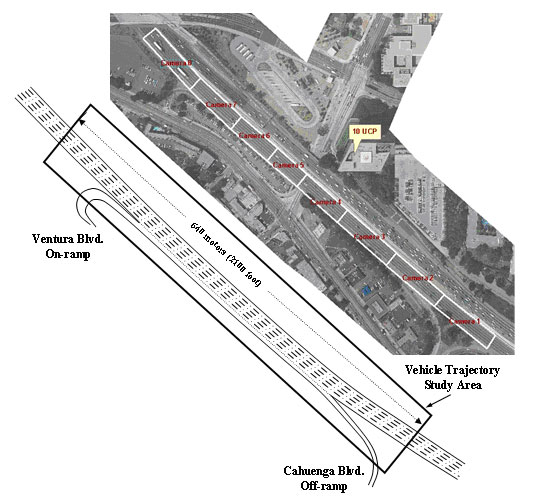
\includegraphics[width=7cm]{./figures/07030fig1.jpg}
\caption{US highway 101}
\label{fig:pict_us80}
\end{center}
\end{figure}



\section{Changes to the original program}


List of the original program and the changes will be inserted.

